%
%  $Description: Author guidelines and sample document in LaTeX 2.09$
%
%  $Author: ienne $
%  $Date: 1995/09/15 15:20:59 $
%  $Revision: 1.4 $
%
\documentclass[10pt,twocolumn]{article}
\usepackage{latex8}
\usepackage{times}
\usepackage{graphicx}
%-------------------------------------------------------------------------
% take the % away on next line to produce the final camera-ready version
%\pagestyle{empty}
%-------------------------------------------------------------------------
\begin{document}
\title{An Experimental Model-Based Rapid Prototyping Environment for High-Confidence Embedded Software}
\author{Joseph Porter, Peter Volgyesi, Nicholas Kottenstette, Harmon Nine, Gabor Karsai, Janos Sztipanovits\\
Institute for Software Integrated Systems \\ Vanderbilt University\\ 2015 Terrace Place, Nashville, TN 37203 USA\\ jporter@isis.vanderbilt.edu\\
}
\maketitle
\thispagestyle{empty}
\begin{abstract}
   The development of embedded software for high-confidence systems is a challenging task that must be supported by a deep integration of control theoretical and computational aspects. Model-based development of embedded software has been practiced for more than a decade now, but very few integrated approaches have emerged to provide end-to-end support for the process, and integrate platform aspects as well as verification. The paper describes an early version of a model-based prototyping toolchain that provides such support and covers most engineering steps. The toolchain is coupled with a hardware-in-the-loop simulation system, allowing quick experimental evaluation of designs. 
\end{abstract}
%-------------------------------------------------------------------------
\Section{Introduction}

Embedded software is a key ingredient in many engineering systems and plays a critical role in providing novel functionality (like advanced controls) while satisfying safety and dependability requirements. Embedded software is also essential for cyber-physical systems where computation is integrated with the physical world. In spite of its importance, development processes and tools today are often ad hoc, and various aspects of engineering are addressed by loosely integrated tools (if they are integrated at all).

The state-of-the-art in the industry today appears to be the use of a model-based tool built on a simulation framework --- Simulink/Stateflow\cite{mathworks:tools} being the prime example. These tools provide a graphical modeling environment (i.e., a block diagram editor), a library of behavioral blocks, a simulation engine, and a code generator for target embedded platforms. However, they fall short in a number of respects, including:

\begin{itemize} 
\item Software architecture modeling is not addressed. Embedded software often contains elements not generated from models. These elements play an important functional role, yet they cannot be expressed as a block in a simulation model. 
\item Timing and schedulability analysis are often missing. The prevailing paradigm for performing the scheduling for embedded software appears to be that of 'trial-and-error', i.e. code gets generated for a platform by a code generator and is deployed by some deployment tool whose details are often hidden from the developer. If the application does not exhibit the desired timing behavior during testing, the designer has to adjust the models (or tweak the generator). 
\item The deployment of functions on the platform is not modeled. Functions must be allocated to computational and communication resources, and this mapping must be done by taking platform behavior and performance constraints into account. 
\item Verification tools are rarely integrated deeply into the development process, though there are initial efforts in this area. This integration is not trivial -- the precise model of computation implicitly used in such tools has to be understood, and design models must be translated into the proper formalisms.
\end{itemize}

In summary, we need better embedded system development toolchains that increase the productivity of the designers via (1) rich modeling capabilities that cover both the functional and non-functional aspects of the design, (2) integrated support for analysis and verification (beyond the already supported simulation). The toolchain has to support a design flow that facilitates moving from models to realistic experimentation and testing, preferably on a platform that contains a high-fidelity replica of the real physical environment. Below, we define some the design aspects that such a toolchain should support.

\begin{enumerate}
    \item \emph{Model-based control system design and analysis problems}. 
When the primary function of embedded software is providing control for a physical system, the control-theoretical analysis and design must be performed first. The designers are control engineers who need to be isolated from particular, platform-specific details as much as possible. This isolation cannot be total, as ultimately the embedded software running on a platform will imperfectly implement an ideal controller. Hence, the control designer must consider some platform abstractions. Furthermore, the actual embedded software has to be evaluated in a physical environment --- not only within a simulation engine. Hardware in the loop simulation is a cost-effective means to test physical compatibility, and should be supported by the tools. 
    \item \emph{Architecture Modeling.}
Functional models of control algorithms must be turned into deployable software components that are executed on a software platform (i.e., an operating system and services deployed on it). Designers have to make decisions about componentization of the functional design, and the design may include components that are not generated from the models. In short, the componentization should also provide support for integrating legacy and non-model-based components. Designers must also be able to describe the hardware platform they use, including its properties and topology. These models need to be taken into consideration when analyzing, scheduling, and deploying the application.
    \item \emph{Schedulability and scheduling.}
When run-time (online) scheduling is used, the embedded software design has to be subjected to schedulability analysis \emph{before} deployment. When design-time (off-line) scheduling is used, the actual schedule has to be generated during the engineering process. These steps are to provide assurances that timing requirements are satisfied by the implementation. In order to validate the design with the timing of the calculated schedule, we use simulation that includes platform-specific details.
    \item \emph{Deployment.}
Logical software design models have to be augmented with deployment models that map components to computational resources and component interactions to communication resources of the software/hardware platform. The same platform could be used for many different applications, hence deployment models must link specific platform concepts to specific software architecture concepts. Note that these models are not merely for documentation, but configuration files and other engineering artifacts must be generated from them to actually support the deployment.
\end{enumerate}    

\begin{figure}[ht]
\centering
%\includegraphics[width=\columnwidth]{figures/starmac_sys.jpg}
%\includegraphics[width=0.9\columnwidth]{figures/starmac_arch_top.pdf}
\includegraphics[width=0.9\columnwidth]{figures/starmac_sys_arch.png}
    \caption{Starmac controller model in Simulink. The dynamics model captures the continuous-time behavior, the IMU (3DM\_GX1) and GPS (SUPERSTAR\_II) blocks model sensors, and the gum\_stix/robo\_stix models contain controller details.}
    \label{fig:starmac}
\end{figure}

A running example in the paper illustrates the use of the toolchain. Fig. \ref{fig:starmac} shows a Simulink model for the Starmac quadrotor helicopter ~\cite{HHWT07}.  The helicopter has a very flexible design for testing onboard computing hardware and sensor options.  One configuration divides computation between a fast, simple inner attitude control loop running on an embedded microcontroller and a slower, more computationally intensive inertial control loop running on a higher-end CPU.  We will describe the model-based development of the respective control software for this configuration.  Distribution over only two processors and a single data bus represents a very simple sample, but one which lends itself to a clear and detailed presentation.  Our results are still preliminary, but we will discuss some of the design problems exposed by the prototype.  We will also cover some related modeling and tool integration efforts.


\Section{Rapid Development Process}
Embedded system development processes are often presented on a ``V-diagram'', such as that shown in Fig. \ref{fig:vdiagram}. On this particular version of the diagram we show software development on one branch, hardware development on the other, and integration in the middle. While building tools to support familiar development processes, we also aim to improve the processes by shortening the length of design, development, and verification cycles.  This is achieved through model-based automation of development steps as well as providing feedback to earlier development stages as analysis results become available.  Our model-based prototyping toolchain models the software architecture (SwA), component design (CD), hardware architecture (HwA), system architecture (SY), and deployment (DPL) stages depicted in the diagram. The design of the modeling language and the toolchain capabilities are described more fully in ~\cite{aces08}.  

\begin{figure}[ht]
\centering
\includegraphics[width=\columnwidth]{figures/dev_diagram.jpg}
    \caption{Development flow for model-based embedded systems design tools}
    \label{fig:vdiagram}
\end{figure}

The development and prototyping process begins with (1) control design (in our case, using Simulink), where the controllers are modeled as hierarchical dataflow networks of function blocks ('subsystems' in Simulink terminology). Next, the subsystem models are elaborated to construct software component models (2), from which a software architecture model is built (3). The hardware platform models (4) describe the hardware architecture, including processors and buses. The software components ('tasks') and component interactions ('messages') are mapped to hardware elements in the deployment model (5). At this point, the suite of models could be subjected to schedulability analysis (6), followed by scheduling (7), and executable code is generated (8) from the functional blocks and the architecture models. The models are also rich enough to perform timing analysis using verification tools (like ~\cite{TrueTime}) The development process can take advantage of a hardware-in-the-loop simulator that is connected to the actually controller hardware. The simulator runs a high-fidelity, real-time dynamic simulation of the controlled 'plant' (a vehicle in our case). 

\begin{figure}[ht]
  \centering
  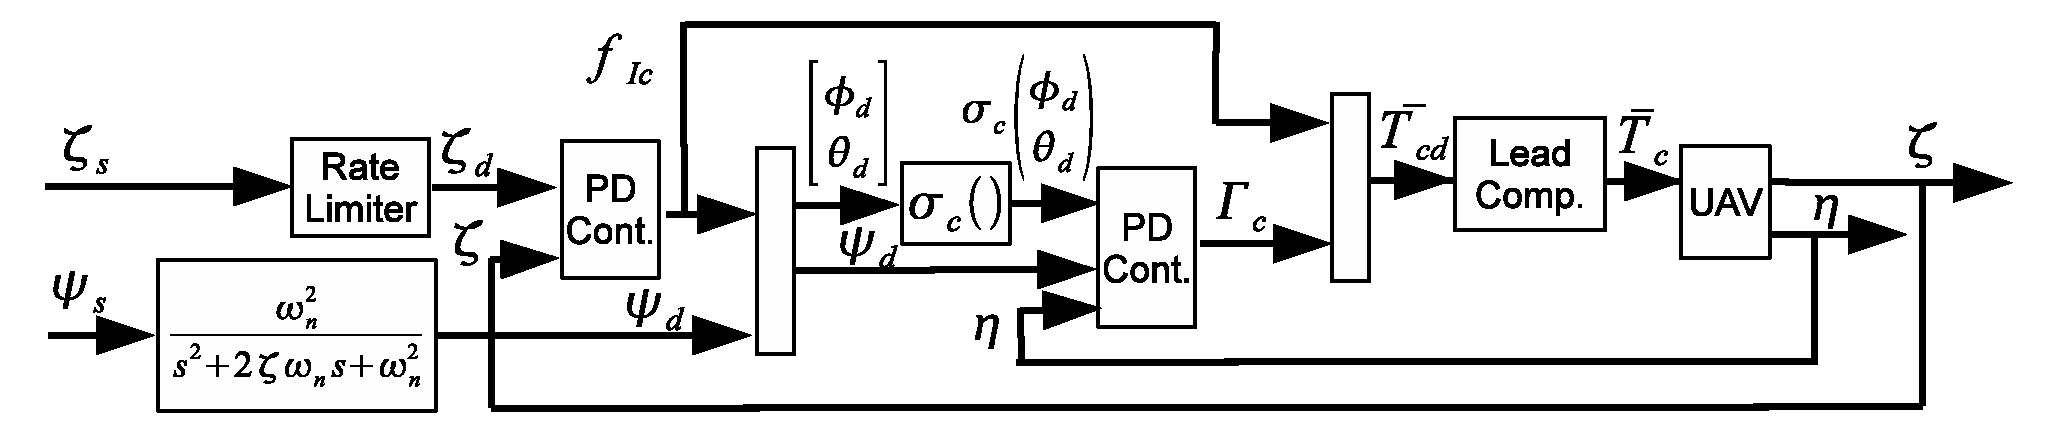
\includegraphics[width=\columnwidth]{figures/high_level_quad_control_sys}
  \caption{High-level quad-rotor control system diagram \cite{NJ:ISIS-08-911}}
  \label{fig:high_level_quad_control_sys}
\end{figure}

\SubSection{Passivity based control design and conic system verification}

Fig.~\ref{fig:high_level_quad_control_sys} depicts the nested control system used to explicitly control the quad-rotor's inertial position $\zeta$ and yaw $\psi$.  The inner control-loop for attitude $\eta = [\phi,\theta,\psi]^\mathtt{T}$ consists of a passive proportional-derivative (PD) controller.  The outer control-loop for $\zeta$ is also a PD controller.  A non-linear mapping based on the system kinematics, desired inertial control force $f_{Ic}$ and desired yaw $\psi_d$ results in a corresponding desired roll $\phi_d$ and pitch $\theta_d$ which were correspondingly limited to the range $[-\frac{\pi}{4},\frac{\pi}{4}]$.  The desired yaw, and range limited roll and pitch depicted respectively as $\psi_d$ and $\sigma_c([\phi_d,\theta_d]^\mathtt{T})$ are inputs to the attitude PD controller in which $\Gamma_c$ is the desired control torque.  However, neither the desired control torque $\Gamma_c$ nor the inertial control force $f_{Ic}$ can be explicitly applied to the quad-rotor aircraft.  Instead, a matrix transformation is used to determine the desired rotor control thrust $\bar{T}_{cd}$.  Finally, in order to compensate for the slow rotor dynamics a passive lead compensator is implemented to determine the corresponding rotor thrust command $\bar{T}_c$ which is sent to the corresponding four rotors on the quad-rotor aircraft (denoted UAV) in the figure.  For additional details the interested reader is referred to \cite{NJ:ISIS-08-911}.

\begin{figure}[ht]
\centering
%\includegraphics[width=\columnwidth]{figures/inertial_control.jpg}
%\includegraphics[width=\columnwidth]{figures/starmac_inertial.pdf}
\includegraphics[width=\columnwidth]{figures/starmac_inertial_controller.png}
    \caption{Simulink model for the nonlinear inertial controller}
    \label{fig:controller}
\end{figure}

Simulink was used to design, test, and verify our controller, including the inertial-control subsystem depicted in Fig.~\ref{fig:controller}.  Simulink's block-based graphical design paradigm is very expressive and intuitive to control designers.  However, nonlinearity and model complexity (i.e., the high degree of interconnection between components) can make such designs difficult to analyze. On the other hand, such safety-critical control systems are examples of the \emph{high-confidence design} paradigm. Aircraft certification authorities require proof (or at least evidence) that controllers, software designs, and implementations meet safety requirements \cite{DO178B}.  Automated verification can be intractable for large designs, so we prefer methods which facilitate \emph{design decoupling}.  Decoupling means that component-level analysis together with adherence to composition rules are sufficient to ensure correct behavior. Here we use passivity based controller design techniques \cite{NJ:ISIS-08-911} to facilitate decoupling. 

Passivity is a good example of a property which facilitates design decoupling.  In control theory, passive systems do not introduce new energy into the overall system.  Furthermore, systems which consist of cascades of two passive systems can be composed using a nested feed-back structure which results in a stable configuration --- in fact, most PD controllers for non-linear passive systems depend on this property \cite{NJ:ISIS-08-911}.  Verifying stability of a network of passive components requires analysis of each component at the local level, with extended joint state space analysis of components connected serially.  A simple topology check is all that is required beyond this.  Passivity may be verified locally for linear components using linear matrix inequalities (LMIs), where a convex optimization problem and associated solver determine whether certain matrix conditions hold.  We are investigating methods to verify sector conditions (for which passivity is a special case) related to stability for both linear and nonlinear systems \cite{NJ:ISIS-08-911}. Our prototyping tools must handle a wide range of designs, including nonlinear designs and complex networks of components.  One reason for choosing the Starmac example was to demonstrate our capabilities with nonlinear models.

\SubSection{Model-Based Design}

Model-based design is performed with the help of design languages that are often graphical. For our environment we have developed a domain-specific modeling language (DSML), ESMoL, that is specified by metamodels using the Generic Modeling Environment\cite{karsai:mic}.  A DSML metamodel restricts design models to structurally correct ones, eliminating large classes of potential errors from a design.  Structural correctness is not sufficient by itself; the DSML must have well-defined behavioral semantics to complete the definition.  For example, Simulink allows a designer to construct models from libraries of functional blocks.  Any properly constructed model can then be simulated to assess the design, so Simulink has a complete behavioral semantics that is defined by the simulation engine.  Note that behavior validated in simulation may change dramatically once the various functions are implemented and deployed on a platform, so additional modeling is required to capture platform effects in control designs. metamodels using the Generic Modeling Environment\cite{karsai:mic}.  A DSML metamodel restricts design models to structurally correct ones, eliminating large classes of potential errors from a design.  Structural correctness is not sufficient by itself; the DSML must have well-defined behavioral semantics to complete the definition.  For example, Simulink allows a designer to construct models from libraries of functional blocks.  Any properly constructed model can then be simulated to assess the design, so Simulink has a complete behavioral semantics that is defined by the simulation engine.  Note that behavior validated in simulation may change dramatically once the various functions are implemented and deployed on a platform, so additional modeling is required to capture platform effects in control designs.

\begin{figure}[ht]
\centering
%\includegraphics[width=\columnwidth]{figures/inertial_control_gme.jpg}
\includegraphics[width=\columnwidth]{figures/starmac_gme.png}
    \caption{ESMoL model for the inertial controller (imported from Simulink)}
    \label{fig:gme_ctrl}
\end{figure}

Models in ESMoL\cite{aces08} describe distributed embedded control systems subject to time-triggered execution semantics.  The time-triggered architecture (TTA) follows a distributed, timed model of computation in which all tasks and message transfers between tasks execute periodically, at pre-calculated time instants\cite{kopetz:2001-22a}. The clocks of computing nodes in the system are tightly synchronized. This technique enables distributed fault-tolerance techniques such as detecting and isolating faulty nodes, and deterministic execution of replicated computations.  Each task has logical execution time semantics\cite{henzinger01giotto}, which means that all input messages are available before a task consuming them is released, and output messages of the task are sent at precisely defined points in time, after the task has finished.  Any task requiring data can not start before the deadline of the sending task plus the transfer time of the message.  Any well-formed ESMoL model has a corresponding time-triggered model of execution whose global behavior may be assessed at design-time, by schedule determination.

ESMoL is a design language that includes the discrete-time subset of Simulink and Stateflow as sub-modeling languages, but it extends those with modeling constructs for componentization, platform modeling, and deployment modeling. It provides an end-to-end approach for connecting the controller models to actual implementation and deployment, where the design engineer has a large freedom in making choices the influence the physical realization of controllers, and has the opportunity to perform various analysis steps in the process.

%\subsubsection*{Import and Architecture model}

\begin{figure}[ht]
\centering
\includegraphics[height=1in]{figures/sw_arch.jpg}
    \caption{ESMoL model for the software component architecture}
    \label{fig:sw_arch}
\end{figure}

\textbf{Import and Architecture Model.} First, the designer imports a Simulink model into the ESMoL modeling tool (built using GME).  Fig. \ref{fig:gme_ctrl} shows an example --- the inertial controller.  The imported dataflow model is a structural replica of the original, though the time-triggered semantics of ESMoL allows use of only Simulink blocks and structures that execute periodically, following a 'clocked-synchronous' model. Subsystems in the GME replica are used to create the components for a software architecture model, as in Fig. \ref{fig:sw_arch}.  Generally, the architecture mimics the structure of the Simulink functional design, possibly with multiple functional block instances or external code fragments added to the component fabric.  Blocks in this diagram correspond to imperative (C) code that will implement the specified functions.  Connections represent either direct synchronous procedure calls between components, or time-triggered messages delivered by the network.

%\subsubsection*{Platform model}

\begin{figure}[ht]
\centering
\includegraphics[height=1in]{figures/platform.jpg}
    \caption{ESMoL model for the computational hardware (Gumstix/Robostix pair)}
    \label{fig:platform}
\end{figure}

\textbf{Platform Model.} In our experimental setup, the hardware for the Starmac control system consists of a Gumstix Verdex embedded processing module, with a Robostix I/O expansion board.  The Gumstix is a PXA-based processing board with both wired and wireless Ethernet as well as expansion connectors.  The Robostix has an Atmega 128 microcontroller with numerous ports for collecting sensor data or providing actuation signals.  One Robostix UART is dedicated to the 'plant' data connection (see below).  An I2C bus links the Gumstix with the Robostix, which exchange sensor, state, and control data.  The ESMoL model of the platform is appropriately simple (Fig. \ref{fig:platform}).

The time-triggered platform is realized in a simple, portable software implementation of the TTA\cite{RT_Thesis}.  The FRODO virtual machine (VM) implements the time-triggered execution of  tasks, and has a communications layer which handles the buffering and timed transfers of data messages.  The current version runs on generic Linux (on the Gumstix) as well as the FreeRTOS (on the AVR).  If a new processor or OS is used, the VM needs to be ported to that new platform. 

%\subsubsection*{Deployment model}

\begin{figure}[ht]
\centering
\includegraphics[width=\columnwidth]{figures/deploy.jpg}
    \caption{ESMoL model for task deployment (center): the outer loop task (top) sends trajectory information to the inner loop task (bottom), which handles sensor data and controls attitude.}
    \label{fig:deploy}
\end{figure}

\textbf{Deployment Model.} The deployment model contains tasks and messages, which connect the software and hardware elements.  Tasks encapsulate software components that execute at the same periodic rate, and assign them to a processing node.  The software components within a task are specified via references ('pointers') to component instances in the software architecture model.  Messages implement the time-triggered communications defined as connections in the software architecture.  Message references connecting tasks ensure that the sender and receiver point to the same message object.  Fig. \ref{fig:deploy} shows the details of the deployment model for our example.

%\subsubsection*{Schedule Computation}

\textbf{Schedule Computation.} Schedule determination is one type of analysis that has been integrated into our rapid development environment.  Fig. \ref{fig:roundtrip} depicts the round-trip scheduling process. A model transformation generates a configuration file for the scheduling tool.  Once run, the scheduling tool internally converts the configuration to finite-domain integer constraint models\cite{offlinescheduling} which are then solved using the Gecode constraint solver tool\cite{gecode}.  If a schedule can be found, then the result is written back into the design model using modeling tool's API.  The running example is trivial --- each processor has only a single task and one message receiver (the other end).  Both tasks execute at the same time, and data transfers can occur immediately after each task deadline on the full-duplex serial link.  Each task invocation gets its data (previously transferred by the virtual machine) from a buffer.

To validate the controller performance with respect to the computed schedule, we use the TrueTime \cite{TrueTime} blocks in Simulink to perform platform-specific resimulation.  TrueTime provides a framework for modeling platforms (processors, networks, scheduling, and protocols), and for exploring the effects of the platform (delays, quantization effects). 

\begin{figure}[ht]
\centering
\includegraphics[width=\columnwidth]{figures/roundtrip.jpg}
    \caption{Integration of the scheduling tool with the modeling environment}
    \label{fig:roundtrip}
\end{figure}

\SubSection{Software synthesis}

Software synthesis creates executable code from well-formed models.  In our tools, code generation occurs at two points: the platform-independent code dealing with the actual (control) functions in the design, and platform-dependent 'glue' code specific to the actual software platform and the chosen model of computation.  This latter includes configuration code, and task wrappers for functional code. For functional code generation we use a graph transformation-based technique \cite{KS:ISIS-04-505}. For platform-specific code we use a simple, template-based code generator that relies on the model access API-s provided by the modeling environment. This generator produces code for task wrappers, message structures, timing information (provided by the scheduler), and configuration. The complete execution environment for the target platform consists all of the generated code, the virtual machine code, and the platform operating system. 

\Section{Hardware-in-the-Loop Simulation}
Hardware-in-the loop (HIL) simulation allows designers to test aspects of the running system using the data interfaces that would be presented to the actual physical device to be controlled (as much as possible) .  Fig. \ref{fig:sim_flow} shows our proposed overall development process for rapidly getting a system working with respect to actual hardware interfaces. The process starts with a fully simulated model, and progresses through steps where simulated elements are incrementally replaced by real implementations, resulting in a fully implemented system. The key idea is that interfaces are preserved throughout, and consistent interface semantics and behavior are maintained across the steps.

\begin{figure}[ht]
\centering
\includegraphics[width=\columnwidth]{figures/sim_flow.jpg}
    \caption{Proposed development process supported by hardware-in-the-loop simulation}
    \label{fig:sim_flow}
\end{figure}

The Mathworks' xPC Target\textregistered tool\cite{mathworks:tools} enables real-time HIL simulation of a model built in Simulink.  The HIL simulation model can be derived from the original (vehicle) simulation model, as shown in Fig. \ref{fig:xpc_sim}. Simulated dynamic systems (plants) must use fixed-step solvers only, and include explicit rate transition blocks where the data rate changes between blocks or subsystems.  Data transfers between the simulated plant and the Robostix controller occur on a serial link which acts as the 'sensor/actuator interface'.  This is a realistic simulation of the physical world, as the actual sensor devices also provide data via serial transfers.  In the figure the control subsystems have been removed and replaced by a block implementing data transfers (upper half). The lower half of the diagram has details for the transfer block and the message marshalling/unmarshalling functions. 

Our initial effort focused on quickly getting from models to a functional system. We used a simplified version of the dynamics to work out the communication and data interface details.  As such, we lack detailed results for performance, reliability, and safety of the generated controllers. However, some useful observations are in order:

\begin{enumerate}
\item Schedule determination attempts to enforce timing restrictions between sensors and actuators, as specified by the designer.  These specifications may be incomplete or infeasible.  The HIL simulation allowed us to quickly see destabilizing schedule effects, allowing us to debug and then validate the schedule.  TrueTime resimulation can also be useful in this regard, but it is less mature in our tools than the HIL simulation.  Our scheduling is not yet fully automated, as hand-tweaking is often necessary.
\item The HIL configuration effectively exposed the lack of synchrony between the sensors and the precisely timed control calculations.  We were forced to add smart buffering code to our virtual machine to ensure that serial transfers from the sensors had completed before attempting to use the data.
\end{enumerate}


\Section{Related Work}

Beyond tools like Simulink, the modeling community has pursued a number of approaches that bring model-driven development toolchains to embedded system development. For example, SysWeaver \cite{sysweaver:niz} includes a modeling tool, import capability for Simulink, code generation, and support for distributed platforms; but does not use the time-triggered model of computation  and thus lacks off-line scheduling capability.  Other tools generally do not include hardware platform modeling and analysis.

%The DECOS toolchain \cite{decos07} combines a number of existing tools (e.g. the TTech tools, SCADE from Esterel Technologies, and others) but the hardware platform modeling and analysis aspects are not covered. 

\begin{figure}[ht]
\centering
\includegraphics[width=\columnwidth]{figures/xpc_model.png}
    \caption{Plant simulation model for Mathworks' xPC Target(R)}
    \label{fig:xpc_sim}
\end{figure}

Similar goals, concepts, tools, and techniques are also found in large standardization efforts and research projects for real-time embedded systems development.  The UML profile for Modeling and Analysis of Real-Time and Embedded systems (MARTE)\cite{marte} provides software modeling tools with a framework for embedded control systems modeling and design.  The Architecture and Analysis Design language (AADL)\cite{AADL} is a textual specification language with similar aims. Projects based on these tools include modeling\cite{Topcased}, schedulability analysis\cite{cheddar}, and verification\cite{aadl_bip}.  Our effort differs in the fundamental approach -- we aim to build up a tool chain and modeling language from the ground up to experiment with design decoupling techniques, rapid integration of heterogeneous tools, and formal semantics.  The language is deliberately kept simple, containing only what we actually use.  Due to its experimental nature some parts of the language and tool infrastructure change very frequently (in contrast with standardized languages and tools).  As it expands we will seek a larger user base and possibly integration with existing tools.



\Section{Conclusion and Future Work}
The presented toolchain is the subject of ongoing research and development. The toolchain is based on the pervasive use of models in the development, and it is targeting a well-defined, robust computational platform based on the time-triggered approach. Design-time scheduling and analysis are important ingredients. The HIL environment provides rapid, realistic experimental evaluation of controller designs. In our applications we have taken advantage of the passivity-based control design techniques that further mitigate the effects of platform uncertainties.  

The original Starmac control software was written in C over approximately four years (as of this writing), including at least three iterations of the control design and platform, as well as extensive testing.  The tools presented here have been in development nearly as long. For the quad-rotor vehicle, the control design, platform customization, model-based redesign, and generation of software (up to the testable point) took approximately three man-months using these prototyping tools.

Promising research avenues, system limitations, and tool deficiencies drive our future efforts.  The controller models have already been extended to include additional features (e.g., yaw control).  Unfortunately, the current implementation is right at the edge of the processing capabilities of the Robostix AVR processor using a floating-point emulation library.  We are considering techniques which can provide validated fixed-point implementations.  Decreasing the sampling frequency is another promising avenue, but which requires serious theoretical analysis to ensure safety.
   
The modeling tools need additional development in requirements capture, as well as more detailed hardware descriptions. Better hardware descriptions will allow us to generate code for devices within the microcontrollers, and to enrich the set of communication media and protocols for which we can generate code.   In particular, platform-dependent communication concepts still need a better representation in the modeling environment.  \cite{aces08} discusses future tool directions in greater detail. 

\Section{Acknowledgements}
This work was sponsored (in part) by the Air Force Office of Scientific Research, USAF, under grant/contract number FA9550-06-0312.  The views and conclusions contained herein are those of the authors and should not be interpreted as necessarily representing the official policies or endorsements, either expressed or implied, of the Air Force Office of Scientific Research or the U.S. Government.

\bibliographystyle{latex8}
\bibliography{rsp09}
\end{document}
